\documentclass{beamer}
\usepackage[utf8]{inputenc}
\usepackage{biblatex}
% \usepackage[document]{ragged2e}
\usetheme{Madrid}
\usecolortheme{default}
\useinnertheme{circles}
\usepackage{paracol}
\usepackage{multirow}
\usepackage{tikz} 
\usetikzlibrary{shapes.geometric,arrows}
\usepackage[algcompatible]{algpseudocode}

\tikzstyle{block} = [rectangle, draw, fill=gray!50, text width=8em, text centered, rounded corners, minimum height=2.2em, minimum width = 8em]
\tikzstyle{line} = [draw, -latex']

\definecolor{Logo1}{rgb}{0.92, 0.21, 0.26}
\definecolor{Logo2}{rgb}{1, 0.44, 0.37}

\setbeamercolor*{palette primary}{bg=Logo1, fg=white}
\setbeamercolor*{palette secondary}{bg=Logo2, fg=white}
\setbeamercolor*{palette tertiary}{bg=white, fg=Logo1}
\setbeamercolor*{palette quaternary}{bg=Logo1,fg=white}
\setbeamercolor{structure}{fg=Logo1} % itemize, enumerate, etc
\setbeamercolor{section in toc}{fg=Logo1} % TOC sections

%------------------------------------------------------------
%This block of code defines the information to appear in the
%Title page
\title[Enhancing Privacy for DASH] %optional
{Enhancing Privacy for DASH-based Video
Streaming}

\subtitle{Evaluation 1}

\author[Group-11, B.tech (NITC)] % (optional)
{Akshith Ananthula - B180457EC \hspace{2em} Kolla Rohith Sai - B180591EC \\ Gv Sai Charan - B180401EC \hspace{2em} Gjr Madhuri - B180697EC \\ \vspace{1em} Guided by \\ \textbf{Dr. Vinay Joseph \\ Dr. Hiran V Nath}}

\institute[] % (optional)
{
  National Institute of Technology Calicut\\
  Department of Electronics and Communication Engineering
}

\date[February 21, 2022] % (optional)
{ February 21, 2022}


\logo{\includegraphics[height=1.2cm]{nitclogo.jpeg}}

\begin{document}

%The next statement creates the title page.
\frame{\titlepage}


%---------------------------------------------------------
%This block of code is for the table of contents after
%the title page
\begin{frame}
\frametitle{Table of Contents}
\tableofcontents
\end{frame}
%---------------------------------------------------------


\section{Introduction}
\begin{frame}{Introduction}
    \begin{itemize}
       \item Now a days there is an increase in network traffic in which video streaming takes up a great proportion. 
        \item Increase in the power of technology having a lot of benefit's but, there is a serious threats to our privacy as well. 
        \item Among the threats one of the serious threat is Network Traffic Analysis.
        \item So why is there a threat?
        \item But the data is encrypted right?
        \item Eavesdropper needs only packet size data for prediction which is the main threat. 
        % \vspace{2.5em}
    \end{itemize}
\end{frame}


% \section{Background and Motivation}
% \begin{frame}{Background and Motivation}
%     \begin{itemize}
%         \item In today’s world, privacy is a big concern to handle and also very much important. 
%         \item In Future we can analyze every thing based on the previous data which is also a valuable asset to maintain.
%         \item By knowing this data one can easily mislead people’s priorities. 
%         \item Eg: A person want to buy a product so he started searching about it in YouTube and watched many videos related to that product. Suppose our eavesdropper collected the data and eavesdropper can use that data and make person to buy a false product and result in scam.
%         % \item Why do we need to think of this privacy threat?\vspace{0.5em}
%         % \item Does this effect a lot of people?\vspace{0.5em}
%         % \item DASH is an adaptive HTTP-based protocol for streaming media over the internet. The technology is used to transport segments of live and on-demand video content from web servers to viewers' devices.\vspace{0.5em}
%         % \item DASH is widely used by popular platforms like YouTube, Prime Video, Netflix etc to deliver video to our browser.\vspace{0.5em}
%     \end{itemize}
% \end{frame}

% \section{Brief about DASH}
\begin{frame}{Brief about DASH}
    \begin{itemize}
        \item DASH stands for Dynamic Adaptive Streaming over HTTP. It is a classic request and reply model.
        \item A DASH video is encoded at various bit rates or multiple quality levels and encoded into small segments of data.
        \item Those segments transmitted in the form of packets. Based on the bandwidth during the interval, the size of the packet is downloaded.
        \item If bandwidth is limited client will request segments from a lower bit rate.
    \end{itemize}
\end{frame}



\begin{frame}{}
    \begin{center}
        \includegraphics[scale=0.35]{blockdiagram.png}\\
        Fig 1: Block Diagram
    \end{center}    
\end{frame}

% \section{Problem Statement}
% \begin{frame}{Problem Statement}
%     Our problem in this project is to
%     \begin{itemize}
%         \item Demonstrate privacy threats for DASH that can be exploited using access to just throughput logs.
%         \item Development of techniques to mitigate the privacy threats which essentially reduce the ease of predicting a video using throughput logs.
%     \end{itemize}
% \end{frame}

\section{Objective}
\begin{frame}{Objective}
    \begin{itemize}
        \item Trace the data efficiently for using it in the algorithm.
        \item Implement an algorithm for making similarity predictions between an unknown trace and the existing traces.
        % \item Employ an algorithm similar for similarity prediction.
        \item Create traces for studying them.
        \item Compare trace with the existing traces and identify it.
        \item Create more traces for expanding and making the algorithm efficient.
    \end{itemize}
\end{frame}


% \section{Work done so far}
% \begin{frame}{Work done so far}
%     \begin{columns}
%         \begin{column}{0.6\textwidth}
%             \begin{itemize}
%                 \item Implemented sniffer for creating traces.
%                 \item Preprocessing of data.
%                 \item Implemented algorithm for similarity prediction.
%                 \item Compared trace with the existing traces and identify it.
%             \end{itemize}
%         \end{column}
%         \begin{column}{0.4\textwidth} 
%             \begin{figure}[h]
%                 \centering
%                 \begin{tikzpicture}[node distance = 1.3cm, auto]
%                     \node [block] (init) {Sniffing};  
%                     \node [block, below of= init](ReadA){Filtering TCP Packets};  
%                     \node [block, below of= ReadA](ReadB){Build traces};  
%                     \node [block, below of = ReadB](Sum){Comparing using algorithm};
%                     \path [line] (init) -- (ReadA);   
%                     \path [line] (ReadA) -- (ReadB);   
%                     \path [line] (ReadB) -- (Sum);
%                 \end{tikzpicture}
%                 % \caption{Flowchart} \label{fig:Flowchart}
%             \end{figure}
%             \begin{center}
%                 Fig 4: Flowchart
%             \end{center}
%         \end{column}
%     \end{columns}
% \end{frame}

\section{Algorithm}
\begin{frame}{Algorithm I}
    \begin{columns}
        \begin{column}{0.5\textwidth}
            \begin{algorithm}
            \scriptsize
            \hline
            \caption{\textbf{Unpack function for creating the trace}}\label{alg:cap}
            \hline
            \begin{algorithmic}
            \Require pcap files
            \Function{Unpack pcap file - getarray}{}\\
              \hspace{1em} Filter TCP packets \\
              \hspace{1em} arr = [ ] \\ 
              \hspace{1em} for each-packet in pcap-file: \\
              \hspace{2em}  arr.append(tcp-segment-size)
            \end{algorithmic}
        \end{algorithm}
        \hline
        
        \begin{algorithm}
            \scriptsize
            \hline
            \caption{\textbf{Comparing two traces}}\label{alg:cap}
            \hline
            \begin{algorithmic}
            \Require Unpack function
            \Function{GetScore}{}\\
                \hspace{1em} arr0 = Unpack('file1.pcap').getarray() \\
                \hspace{1em} arr1 = Unpack('file2.pcap').getarray() \\
                \hspace{1em} if size of arrays are different : \\
                \hspace{2em} sample and redistribute the highest sized array \\
                \hspace{1em} compare array's and generate score.
            \end{algorithmic}
        \end{algorithm}
        \hline
        \end{column}
        \begin{column}{0.5\textwidth}
            \begin{center}
                \includegraphics[scale=0.14]{subplot_stanford.png} \\
                \footnotesize Fig 2: Captured logs for video1.
            \end{center}
            \vspace{0.3em}
            \textbf{Observations}: \\
            Similarity percentage got is 28.58 \%.
        \end{column}
    \end{columns}
\end{frame}

\begin{frame}{Algorithm II}
    \begin{columns}
        \begin{column}{0.5\textwidth}
             % In this method, we divide the entire trace into n chunks and then we calculate how many packets for each chunk and then the traces compared using these data.
            \begin{algorithm}
                \scriptsize
                \hline
                \caption{\textbf{Unpack function for creating the trace}}\label{alg:cap}
                \hline
                \begin{algorithmic}
                \Require pcap files
                \Function{Unpack pcap file - getarray}{}\\
                  \hspace{1em} Filter TCP packets \\
                  \hspace{1em} arr = [ ] \\ 
                  \hspace{1em} for each-packet in pcap-file: \\
                  \hspace{2em} arr.append(tcp-segment-size) \\
                  \hspace{1em} Divide the entire trace into n chunks and calculate how many \\
                  \hspace{1em} packets required for each chunk and store it in resultarray.
                \end{algorithmic}
            \end{algorithm}
            \hline
            \begin{algorithm}
                \scriptsize
                \hline
                \caption{\textbf{Comparing two traces}}\label{alg:cap}
                \hline
                \begin{algorithmic}
                \Require Unpack function
                \Function{GetScore}{}\\
                    \hspace{1em} arr0 = Unpack('file1.pcap').getarray() \\
                    \hspace{1em} arr1 = Unpack('file2.pcap').getarray() \\
                    \hspace{1em} compare array's and generate score.
                \end{algorithmic}
            \end{algorithm}
            \hline
        \end{column}
        \begin{column}{0.5\textwidth}
            \begin{center}
                \includegraphics[scale=0.14]{subplot_stanford_m2.png} \\
                \footnotesize Fig 3: Captured logs for video1
            \end{center}
            \vspace{0.3em}
            \textbf{Observations}: \\
            Similarity percentage got is 73.88 \%.
        \end{column}
    \end{columns}
\end{frame}

\begin{frame}{Algorithm III}
    \begin{columns}
        \begin{column}{0.5\textwidth}
            % In this method, we divide the entire trace into n chunks and then we calculate how much time taken for each chunk to arrive and then the traces compared using these data.
            \begin{algorithm}
                \scriptsize
                \hline
                \caption{\textbf{Unpack function for creating the trace}}\label{alg:cap}
                \hline
                \begin{algorithmic}
                \Require pcap files
                \Function{Unpack pcap file - getarray}{}\\
                  \hspace{1em} Filter TCP packets \\
                  \hspace{1em} arr = [ ] \\ 
                  \hspace{1em} for each-packet in pcap-file: \\
                  \hspace{2em} arr.append(tcp-segment-size) \\
                  \hspace{1em} Divide the entire trace into n chunks and calculate how much \\
                  \hspace{1em} time taken for each chunk to arrive and store it in resultarray.
                \end{algorithmic}
            \end{algorithm}
            \hline
            \begin{algorithm}
                \scriptsize
                \hline
                \caption{\textbf{Comparing two traces}}\label{alg:cap}
                \hline
                \begin{algorithmic}
                \Require Unpack function
                \Function{GetScore}{}\\
                    \hspace{1em} arr0 = Unpack('file1.pcap').getarray() \\
                    \hspace{1em} arr1 = Unpack('file2.pcap').getarray() \\
                    \hspace{1em} compare array's and generate score.
                \end{algorithmic}
            \end{algorithm}
            \hline
        \end{column}
        \begin{column}{0.5\textwidth}
            \begin{center}
                \includegraphics[scale=0.14]{subplot_stanford_m3.png} \\
                \footnotesize Fig 4: Captured logs for video1
            \end{center}
            \vspace{0.3em}
            \textbf{Observations}: \\
            Similarity percentage got is -3.35 \%.
        \end{column}
    \end{columns}
\end{frame}

\section{Results}
\begin{frame}[allowframebreaks]{Results}
    \begin{columns}
        \begin{column}{0.5\textwidth}
            \begin{center}
                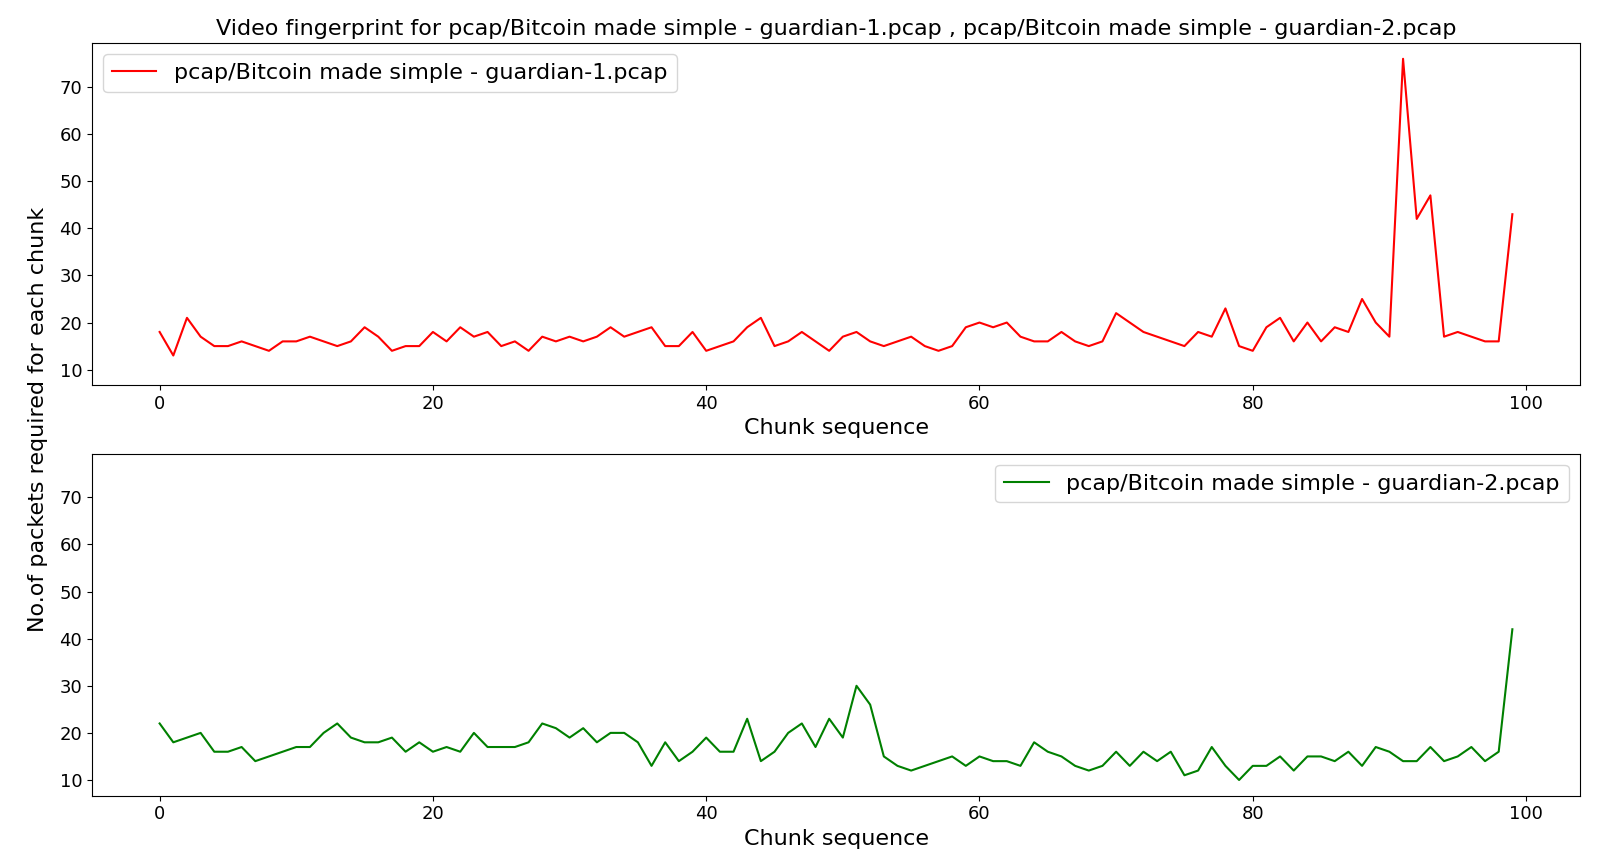
\includegraphics[scale=0.14]{comp_Bitcoin.png} \\
                \footnotesize Fig 4: Captured logs for video2
            \end{center}
        \end{column}
        \begin{column}{0.5\textwidth}
            \begin{center}
                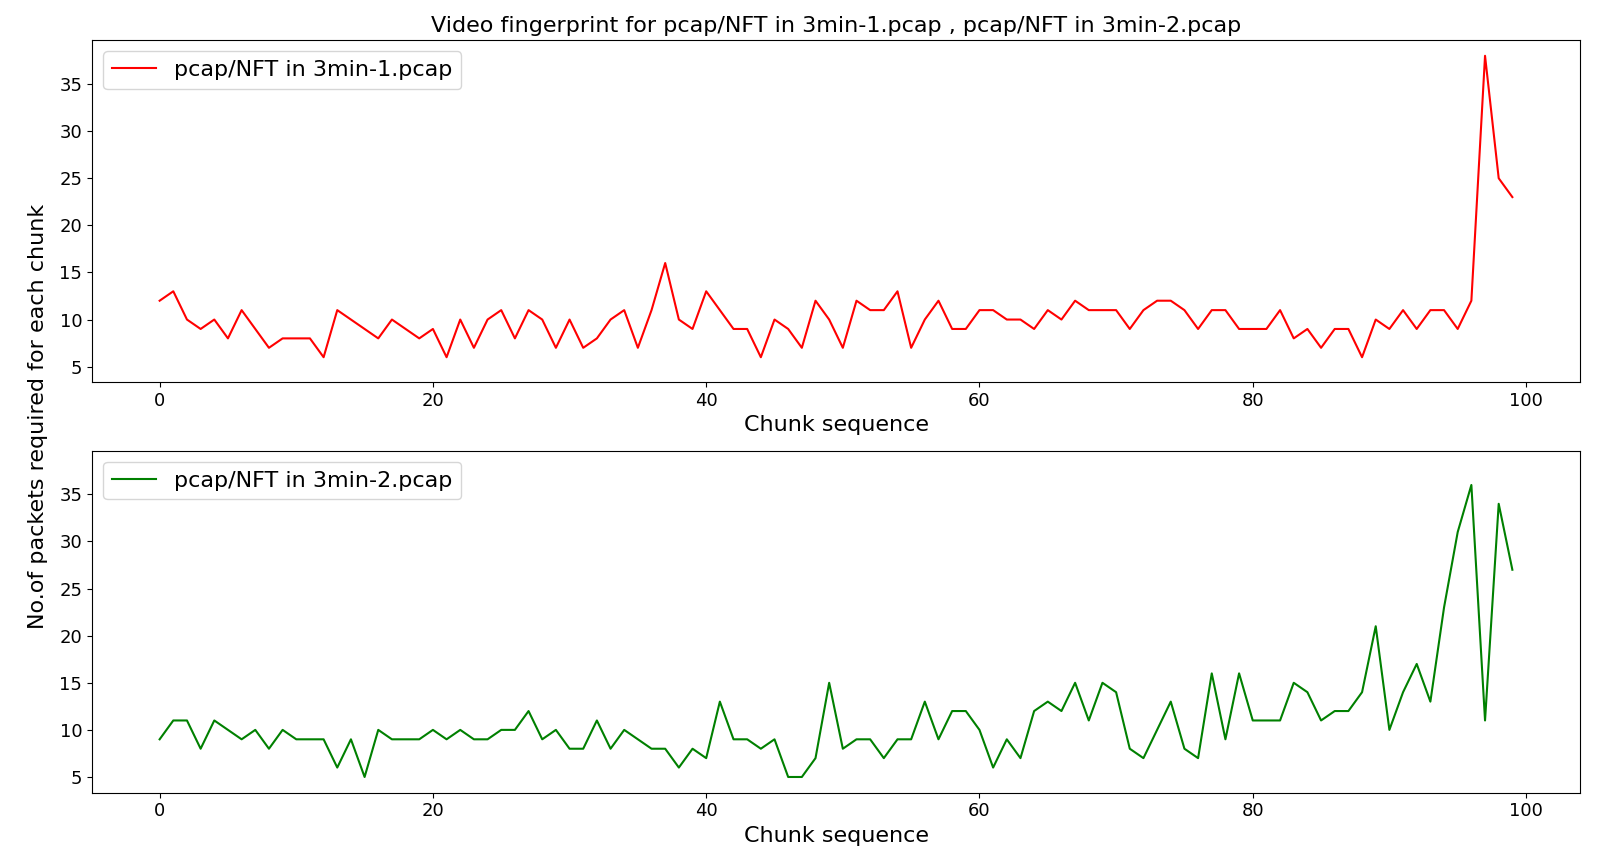
\includegraphics[scale=0.14]{comp_NFT.png} \\
                \footnotesize Fig 4: Captured logs for video3
            \end{center}
        \end{column}
    \end{columns}
    \textbf{Observations}: \\
    \vspace{0.3em}
    \begin{columns}
        \begin{column}{0.5\textwidth}
            Similarity percentage got is 73.94 \%.
        \end{column}
        \begin{column}{0.5\textwidth}
            Similarity percentage got is 64.20 \%.
        \end{column}
    \end{columns}
    
    \newpage
    
    \begin{center}
        \begin{tabular}{ |p{1.5cm}|p{2cm}|p{2cm}|  }
            \hline
            Method & Offline(secs) & Online(secs) \\
            \hline
            VR & 0 & 0.8421 \\
            VUR & 0 & 3.8627 \\
            RR & 163.2745 & 81.4735 \\
            CRR & 38.05965 & 81.4735 \\
            DRR & 3054.6124 & 83.9267 \\
            SR & 38.05965 & 10.176 \\
            \hline
        \end{tabular} 
        \\ \vspace{0.5cm} Table 2.Computation time taken for different methods.
    \end{center}
\end{frame}


% \begin{frame}{Results cont'd}
%     When we compared a trace of levitating video trace with other levitating video trace and also two other video traces present, we got the result as shown. The result was correct but it's missing the prediction accuracy.
%     \begin{center}
%         \includegraphics[scale=0.445]{compare.png}\\
%         Fig 13: Results when tested levitating-0 with others.
%     \end{center}
% \end{frame}


\section{Inferences from results}
\begin{frame}{Inference from results}
    Based on the results we have got the inferences we got are:
    \begin{itemize}
        \item Algorithm 1 is still like the old one which was proposed earlier but the accuracy is further decreased which can be understood by the fact that the data is spread and when two different videos are compared then, the result is far from 2 same videos which can be taken as advantage.
        \item Algorithm 2 is giving good results both with similar and non-similar videos.
        \item Algorithm 3 had bad results which we can understand by the fact that the speed of the connection changes.
    \end{itemize}
\end{frame}



\section{Future plans}
\begin{frame}{Future plans}
    Based on what results in we have got we wanted to choose method 2 (or) algorithm 2 and proceed with mitigating this issue of recognition.  \\ \vspace{1em} For that we read some papers and the ideas we got are:
    \begin{itemize}
        \item Padding the receiving packets shows the reduction of accuracy to 8\%.
        \item Using 802.11n standard that uses multiple antennas to increase data rates which is similar to MIMO hence the data can be bad.
    \end{itemize} 
\end{frame}






\section{References}
\begin{frame}[allowframebreaks]{References}
    \footnotesize \color{black}
    \begin{thebibliography}{100}
        \bibitem{b1} \color{black} A. Reed and B. Klimkowski, "Leaky streams: Identifying variable bitrate DASH videos streamed over encrypted 802.11n connections," \textit{2016 13th IEEE Annual Consumer Communications & Networking Conference (CCNC)}, 2016, pp. 1107-1112, doi: 10.1109/CCNC.2016.7444944.
        
        \bibitem{b2} \color{black} Z. Li, M. A. Kaafar and a. G. Xie, "Session Throughput Prediction for Internet Videos," in \textit{IEEE Communications Magazine}, vol. 54, no. 12, pp. 152-157, December 2016, doi: 10.1109/MCOM.2016.1600386CM.
        
        \bibitem{b2} \color{black} Marc Liberatore and Brian Neil Levine. 2006. Inferring the source of encrypted HTTP connections. In Proceedings of the 13th ACM conference on Computer and communications security (CCS '06). Association for Computing Machinery, New York, NY, USA, 255–263. DOI:https://doi.org/10.1145/1180405.1180437
        
        \bibitem{b4} \color{black} J. Gu, J. Wang, Z. Yu and K. Shen, "Walls Have Ears: Traffic-based Side-channel Attack in Video Streaming," \textit{IEEE INFOCOM 2018 - IEEE Conference on Computer Communications,} 2018, pp. 1538-1546, doi: 10.1109/INFOCOM.2018.8486211. 
        
        \bibitem{github repo} \color{black}https://github.com/akshith6212 

        \bibitem{leaky2} \color{black}Andrew Reed and Michael Kranch. 2017. Identifying HTTPS-Protected Netflix Videos in Real-Time. In Proceedings of the Seventh ACM on Conference on Data and Application Security and Privacy (CODASPY '17). Association for Computing Machinery, New York, NY, USA, 361–368. DOI:https://doi.org/10.1145/3029806.3029821 
    
        \bibitem{ref8} \color{black}George Dean Bissias, Marc Liberatore, David Jensen, and Brian Neil Levine. 2005. Privacy vulnerabilities in encrypted HTTP streams. In Proceedings of the 5th international conference on Privacy Enhancing Technologies (PET'05). Springer-Verlag, Berlin, Heidelberg, 1–11. DOI:https://doi.org/10.1007/11767831\_1 
        
        \bibitem{ref9} \color{black}C. E. Kement, B. Tavli, H. Gultekin and H. Yanikomeroglu, "Holistic Privacy for Electricity, Water, and Natural Gas Metering in Next Generation Smart Homes," in \textit{IEEE Communications Magazine}, vol. 59, no. 3, pp. 24-29, March 2021, doi: 10.1109/MCOM.001.2000263. 
        
        \bibitem{video-stanford} \color{black}https://www.youtube.com/watch?v=UF8uR6Z6KLc
        
        \bibitem{video-levitating} \color{black}https://www.youtube.com/watch?v=TUVcZfQe-Kw
    \end{thebibliography}
\end{frame}

\begin{frame}
    \vspace{1em}
    \centering \huge Thank You!
\end{frame}

\end{document}

% \begin{frame}{Results I}
%     % Using the algorithm mentioned we have tried running it for two videos by which we got some results.
%     \begin{columns}
%         \begin{column}{0.5\textwidth}
%             \begin{center}
%                 \includegraphics[scale=0.14]{subplot_levitating.png} \\
%                 Fig 5: Captured logs for capture-0
%             \end{center}
%         \end{column}
%         \begin{column}{0.5\textwidth} 
%             \begin{center}
%                 \includegraphics[scale=0.14]{subplot_stanford.png} \\
%                 Fig 6: Captured logs for capture-1
%             \end{center}
%         \end{column}
%     \end{columns}
%     \vspace{1em}
%     Observations: 
%     \begin{columns}
%         \begin{column}{0.5\textwidth}
%             \begin{itemize}
%                 \item Similarity percentage got is 28.65 \%.
%             \end{itemize}
%         \end{column}
%         \begin{column}{0.5\textwidth} 
%             \begin{itemize}
%                 \item Similarity percentage got is 28.58 \%.
%             \end{itemize}
%         \end{column}
%     \end{columns}
% \end{frame}


% \begin{frame}{Results II}
%     % Using the algorithm mentioned we have tried running it for two videos by which we got some results.
%     \begin{columns}
%         \begin{column}{0.5\textwidth}
%             \begin{center}
%                 \includegraphics[scale=0.14]{subplot_levitating_m2.png} \\
%                 Fig 5: Captured logs for capture-0
%             \end{center}
%         \end{column}
%         \begin{column}{0.5\textwidth} 
%             \begin{center}
%                 \includegraphics[scale=0.14]{subplot_stanford_m2.png} \\
%                 Fig 6: Captured logs for capture-1
%             \end{center}
%         \end{column}
%     \end{columns}
%     \vspace{1em}
%     Observations: 
%     \begin{columns}
%         \begin{column}{0.5\textwidth}
%             \begin{itemize}
%                 \item Similarity percentage got is 58.08 \%.
%             \end{itemize}
%         \end{column}
%         \begin{column}{0.5\textwidth} 
%             \begin{itemize}
%                 \item Similarity percentage got is 73.88 \%.
%             \end{itemize}
%         \end{column}
%     \end{columns}
% \end{frame}

% \begin{frame}{Results III}
%     % Using the algorithm mentioned we have tried running it for two videos by which we got some results.
%     \begin{columns}
%         \begin{column}{0.5\textwidth}
%             \begin{center}
%                 \includegraphics[scale=0.14]{subplot_levitating_m3.png} \\
%                 Fig 5: Captured logs for capture-0
%             \end{center}
%         \end{column}
%         \begin{column}{0.5\textwidth} 
%             \begin{center}
%                 \includegraphics[scale=0.14]{subplot_stanford_m3.png} \\
%                 Fig 6: Captured logs for capture-1
%             \end{center}
%         \end{column}
%     \end{columns}
%     \vspace{1em}
%     Observations: 
%     \begin{columns}
%         \begin{column}{0.5\textwidth}
%             \begin{itemize}
%                 \item Similarity percentage got is -18.81 \%.
%             \end{itemize}
%         \end{column}
%         \begin{column}{0.5\textwidth} 
%             \begin{itemize}
%                 \item Similarity percentage got is -3.31 \%.
%             \end{itemize}
%         \end{column}
%     \end{columns}
% \end{frame}